\documentclass[tikz,border=10pt]{standalone}
\usetikzlibrary{calc, shapes.geometric, arrows, positioning}
\begin{document}
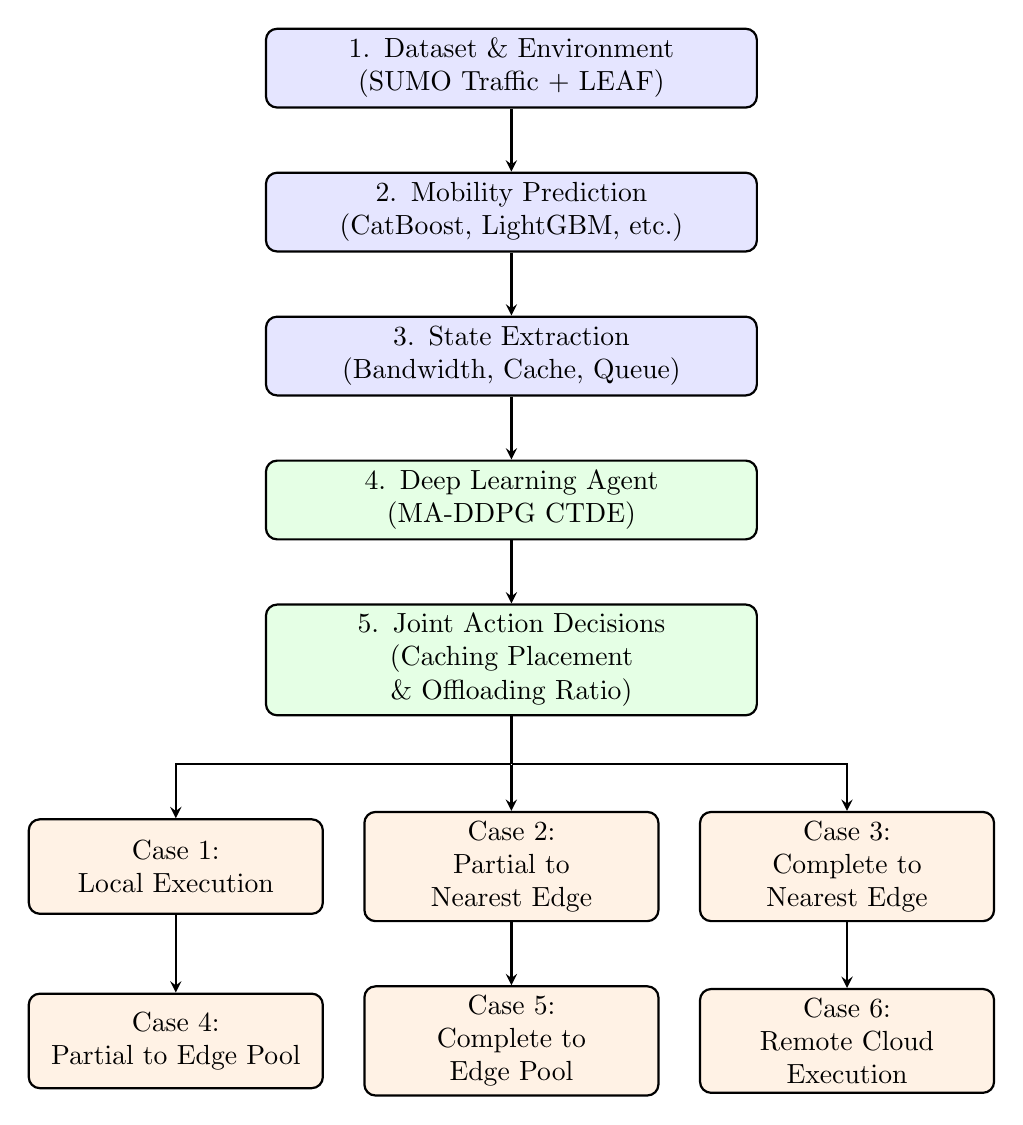
\begin{tikzpicture}[
    node distance=0.8cm and 0.5cm,
    process/.style={rectangle, draw=black, thick, fill=blue!10, text width=6cm, align=center, rounded corners, minimum height=1cm},
    decision/.style={rectangle, draw=black, thick, fill=green!10, text width=6cm, align=center, rounded corners, minimum height=1cm},
    cases/.style={rectangle, draw=black, thick, fill=orange!10, text width=3.5cm, align=center, rounded corners, minimum height=1.2cm},
    arrow/.style={thick, ->, >=stealth}
]

% Top pipeline
\node (dataset) [process] {1. Dataset \& Environment\\(SUMO Traffic + LEAF)};
\node (mobility) [process, below=of dataset] {2. Mobility Prediction\\(CatBoost, LightGBM, etc.)};
\node (state) [process, below=of mobility] {3. State Extraction\\(Bandwidth, Cache, Queue)};
\node (agent) [decision, below=of state] {4. Deep Learning Agent\\(MA-DDPG CTDE)};
\node (action) [decision, below=of agent] {5. Joint Action Decisions\\(Caching Placement \& Offloading Ratio)};

% An intermediate node for routing
\node (dispatch) [below=0.6cm of action, inner sep=0, minimum size=0] {};

% Row 1 of cases
\node (case2) [cases, below=1.2cm of action] {Case 2:\\Partial to Nearest Edge};
\node (case1) [cases, left=of case2] {Case 1:\\Local Execution};
\node (case3) [cases, right=of case2] {Case 3:\\Complete to Nearest Edge};

% Row 2 of cases
\node (case5) [cases, below=of case2] {Case 5:\\Complete to Edge Pool};
\node (case4) [cases, left=of case5] {Case 4:\\Partial to Edge Pool};
\node (case6) [cases, right=of case5] {Case 6:\\Remote Cloud Execution};

% Connect pipeline
\draw [arrow] (dataset) -- (mobility);
\draw [arrow] (mobility) -- (state);
\draw [arrow] (state) -- (agent);
\draw [arrow] (agent) -- (action);

% Connect to cases
\draw [thick] (action.south) -- (dispatch);
\draw [arrow] (dispatch) -| (case1.north);
\draw [arrow] (dispatch) -- (case2.north);
\draw [arrow] (dispatch) -| (case3.north);

\draw [arrow] (case1.south) -- (case4.north);
\draw [arrow] (case2.south) -- (case5.north);
\draw [arrow] (case3.south) -- (case6.north);

\end{tikzpicture}
\end{document}
